\documentclass[tikz,border=6pt]{standalone}
\usepackage[utf8]{inputenc}
\usetikzlibrary{positioning,arrows.meta,fit,calc}
\begin{document}
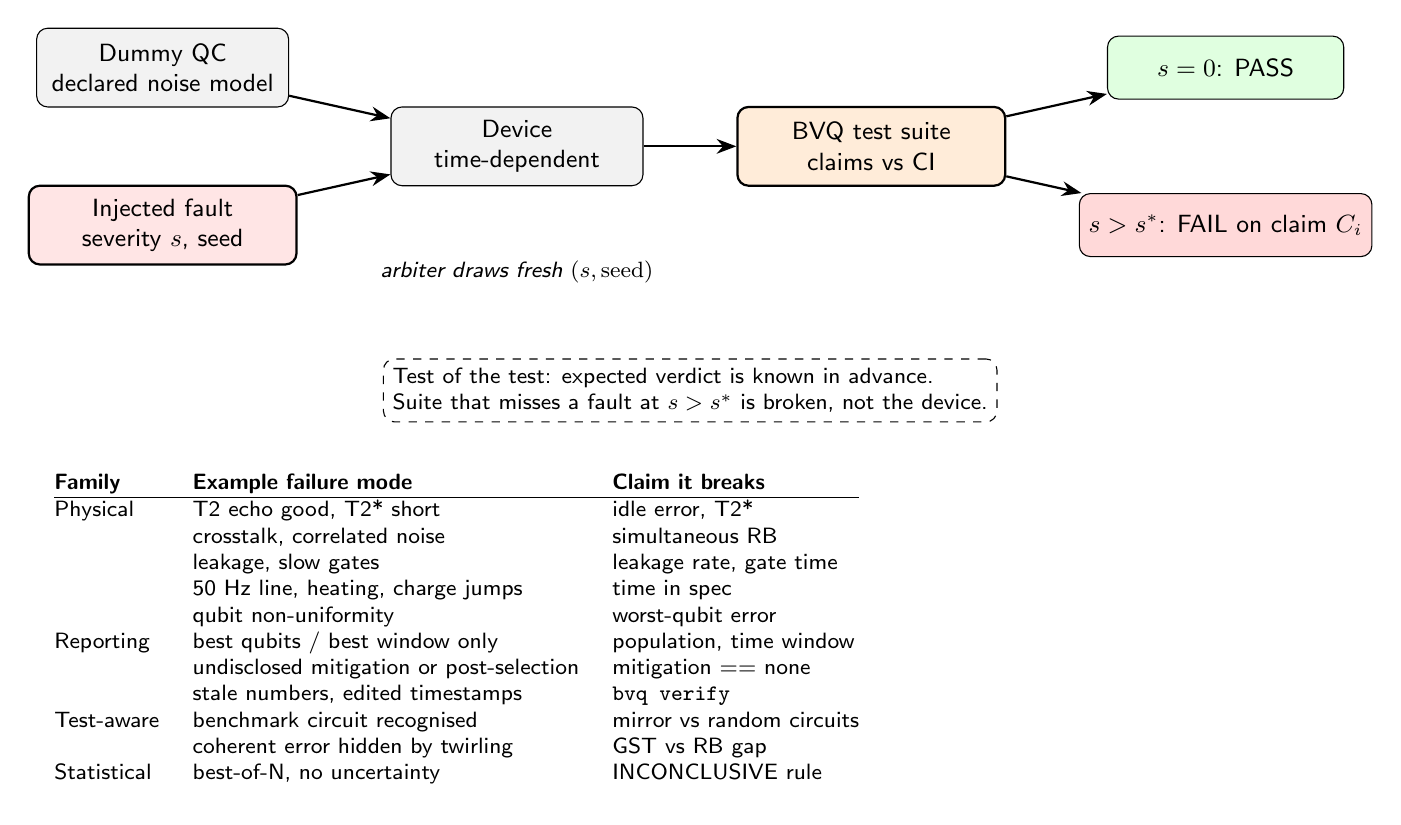
\begin{tikzpicture}[
  font=\sffamily\small,
  box/.style={draw,rounded corners,fill=gray!10,minimum width=3.2cm,minimum height=1.0cm,align=center},
  hot/.style={draw,thick,rounded corners,fill=red!10,minimum width=3.4cm,minimum height=1.0cm,align=center},
  tool/.style={draw,thick,rounded corners,fill=orange!15,minimum width=3.4cm,minimum height=1.0cm,align=center},
  ok/.style={draw,rounded corners,fill=green!12,minimum width=3.0cm,minimum height=0.8cm,align=center},
  bad/.style={draw,rounded corners,fill=red!15,minimum width=3.0cm,minimum height=0.8cm,align=center},
  arr/.style={-{Stealth[length=2.5mm]},thick},
  lab/.style={font=\sffamily\footnotesize\itshape,fill=white,inner sep=1pt}
]
% loop
\node[box]  (base) at (0,0)   {Dummy QC\\declared noise model};
\node[hot]  (fault) at (0,-2) {Injected fault\\severity $s$, seed};
\node[box]  (dev) at (4.5,-1) {Device\\time-dependent};
\node[tool] (suite) at (9,-1) {BVQ test suite\\claims vs CI};
\node[ok]   (pass) at (13.5,0) {$s=0$: PASS};
\node[bad]  (fail) at (13.5,-2) {$s>s^*$: FAIL on claim $C_i$};
\draw[arr] (base) -- (dev);
\draw[arr] (fault) -- (dev);
\draw[arr] (dev) -- (suite);
\draw[arr] (suite) -- (pass);
\draw[arr] (suite) -- (fail);
\node[lab] at (4.5,-2.6) {arbiter draws fresh $(s,\mathrm{seed})$};

% oracle line
\node[draw,dashed,rounded corners,align=left,font=\sffamily\footnotesize] at (6.7,-4.1)
  {Test of the test: expected verdict is known in advance.\\
   Suite that misses a fault at $s>s^*$ is broken, not the device.};

% gallery table
\node[anchor=north west,align=left,font=\sffamily\footnotesize] at (-1.5,-5.0) {%
\begin{tabular}{@{}lll@{}}
\textbf{Family} & \textbf{Example failure mode} & \textbf{Claim it breaks}\\\hline
Physical & T2 echo good, T2* short & idle error, T2*\\
 & crosstalk, correlated noise & simultaneous RB\\
 & leakage, slow gates & leakage rate, gate time\\
 & 50 Hz line, heating, charge jumps & time in spec\\
 & qubit non-uniformity & worst-qubit error\\
Reporting & best qubits / best window only & population, time window\\
 & undisclosed mitigation or post-selection & mitigation == none\\
 & stale numbers, edited timestamps & \texttt{bvq verify}\\
Test-aware & benchmark circuit recognised & mirror vs random circuits\\
 & coherent error hidden by twirling & GST vs RB gap\\
Statistical & best-of-N, no uncertainty & INCONCLUSIVE rule\\
\end{tabular}};
\end{tikzpicture}
\end{document}
